\section{فصل اول}

\subsection{اصطلاحات}

\subsubsection{\lr{World problem} یا \lr{Environment}}

دنیای مسئله جایی است که مشکلی در آن رخ داده است و کسی وجود دارد که این مشکل را
در ابتدا بررسی و بعد از آن حل می‌کند. در حقیقت دنیا، محیط عملیاتی ما در مهندسی
نیازمندی است. این دنیا می‌تواند سینما باشد یا دانشگاه. جنس این مسائل می‌تواند
مشکل باشد که بایستی برطرف شود یا قابلیتی که می‌خواهیم در آینده اتفاق بیوفتد.

\subsubsection{\lr{Machine}}

ماشین راه‌حلی برای حل مسئله‌ای می‌باشد که پیش آمده است. ماشین می‌تواند به صورت
آماده خریداری شود یا توسط تیم توسعه از صفر توسعه داده شود. ما باید در سند
نیازمندی این نوع از نیازمندی را مشخص کنیم. ماشین در حقیقت نرم‌افزاری است که قرار
است داشته باشیم \footnote{\lr{Software to be}}. مدیر نیازمندی با توجه به هزینه
می‌تواند برای مهندس نیازمندی تعیین کند که آیا داشتن نرم‌افزار آماده هزینه کمتری
برایش دارد یا توسعه آن نرم‌افزار از صفر توسط تیم توسعه خود.

\subsubsection{\lr{Context}}

کلمه \lr{Context} به معنای زمینه می‌باشد. تمام رفتار‌ها و شکل‌های انجام کار را
نشان می‌دهد. مشخص می‌کند که چه نیازمندی‌های علمی را باید بدانیم تا بتوانیم در
نرم‌افزار آن را پیاده‌سازی کنیم. زمینه‌های مرتبطی برای توسعه‌ که باید به علوم
آنها واقف شویم. برای مثال هنگام توسعه یک نرم‌افزار تشخیص پیوند مولکولی و طراحی
پروتئین نیازمند آن هستیم که در مورد شاخه‌های علمی بایولوژی، بایوتک و ژنتیک علومی
را کسب کنیم. این علوم می‌تواند توسط تحقیقات و پژوهش‌های فردی بدست آید یا اینکه
در راستای تحصیل در یک رشته می‌توانیم در رشته دیگر به تحصیلات آکادمیک بپردازیم و
به نوعی مدرک کارشناسی آن حوزه را بدست آوریم که بتوانیم به صورت کامل روی موضوع
عملیاتی خود واقف و مسلط شویم.

\subsubsection{\lr{Statement} یا جمله}

\lr{Statement} یک جملست که ترکیبی از پدیده‌ها می‌باشد. برای مثال گفته می‌شود،
وقتی ترمز خودرو فشرده شد، در‌ها قفل شود و کاربر بتواند وضعیت دنده خود را تغییر
دهد. بعضی از این پدیده‌ها در دنیای مسئله یا محیط اتفاق می‌افتد. فعل‌های محیطی را
به هم متصل می‌کند و به فعل‌های نرم‌افزاری دخالتی ندارد.

نکته: کیفیت جمله‌ها لزومی ندارد که درست باشند و می‌توانند مورد نقدر قرار گیرند.

\subsubsection{\lr{Phenomena} یا پدیده‌ها}

تمام اتفاقاتی که در مسئله (یا جمله) رخ می‌دهد را پدیده یا \lr{Phenomena} گویند.
برخی پدیده‌ها دقیقاً داخل نرم‌افزار رخ می‌دهد، مانند خطای TLS یا خطای پیدا نشدن
صفحه. برخی پدیده‌ها بین ارتباطات رخ می‌دهد مانند نرمال‌سازی دیتابیس. پدیده خرید
کردن یک پدیده محیطی است. وقتی برای کاربر اعلانی ارسال می‌شود در واقع این اعلانات
پدیده‌ بین محیط و نرم‌افزار است.

\subsubsection{\lr{System as is}}

سیستمی که در حال حاضر وجود دارد سیستم جاری یا \lr{System as is} گویند. سیستم
جاری بیشتر به محیط مربوط است. به عبارتی دیگر، المان‌ها و ارتباطاتی است که الان
وجود دارد مانند افراد و دستگاه‌ها.

\subsubsection{\lr{System to be}}

\lr{System to be} دقیقاً سیستمی است که در آینده خواهیم داشت. تمام فرایند مهندسی
که منجر به تولید سیستمی جدید می‌شود. چیزی که باید رخ دهد. مجموعه‌ای از المان‌های
محیطی و \lr{Software to be}.

\subsubsection{عوامل \lr{Prescriptive}}

عواملی که تجویزی هستند که نیاز سیستم را مشخص می‌کنند که چه کاری باید انجام شود:

\begin{enumerate}
    \item \lr{System requirement}: یک \lr{System requirement} مجموعه‌ای از
    \lr{Assumption}ها و \lr{Software requirement}هاست. تمام تک کار‌های کوچکی که
    به محیط اختصاص می‌دهیم.
    \item \lr{Software requirement}: تمام نیازمندی‌های نرم‌افزاری که می‌تواند به
    دو دسته \lr{Functional} و \lr{Non-functional} تقسیم شود. تمام تسک‌های کوچکی
    که به نرم‌افزار اختصاص می‌دهیم.
    \item \lr{Assumption}: تمام عوامل محیطی که در پایین توضیح داده شده است.
\end{enumerate}

مثال‌هایی از انواع \lr{System requirement}:

\begin{itemize}
    \item تمام در‌های قطار بایستی در هنگام حرکت بسته باشند.
    \item مشتریان هیچ وقت نمی‌توانند بیشتر از سه کتاب را در یک زمان قرض بگیرند.
    \item تمام محدودیت‌های دعوت یک شرکت کننده به یک میتنینگ آنلاین بایستی به
    زودی برطرف شود.
\end{itemize}

\subsubsection{مفروضات یا \lr{Assumption}}

تمام عواملی که محیطی هستند و مستقیماً با نرم‌افزار ارتباطی ندارند. در واقعیت امر
همان محیط و یا \lr{World problem} هستند. ابزار‌هایی واسط بین انسان و انجام کار.

\begin{enumerate}
    \item \lr{People}: مردم و کاربران
    \item \lr{Device}: دستگاه‌ها مانند سنسور‌ها، جمع‌آور داده و ارسال کننده به
    موتور تحلیل (نرم‌افزار)
    \item \lr{Exists softwares} نرم‌افزار‌های موجود: نرم‌افزار‌هایی که خودشان
    عملیات متعددی انجام می‌دهند و داده‌ها را برای تحلیل به نرم‌افزار اصلی سیستم
    ما ارسال می‌کنند.
\end{enumerate}

عوامل محیطی گسترده هستند. برای مثال وقتی که کاربر در اپلیکیشن سبد خرید خود را
می‌خواهد حساب کند، زدن روی دکمه "پرداخت آنلاین" کاملا یک عامل محیطی است یعنی
\lr{Assumption}. زیرا با دخالت کاربر می‌توان سبد خرید را پرداخت کرد، در غیر این
صورت نرم‌افزار خودش نمی‌تواند تصمیم بگیرد که پرداخت نهایی را کی باید انجام دهد
(دیدگاه یک سیستم ساده).

\subsubsection{مثال}

سناریو: در‌های قطار موقع حرکت قفل شود. در این سناریو \lr{Statement}، پدیده‌ها
(Phenomena) و نیازمندی سیستم و پدیده‌های محیطی را مشخص کنید.

\begin{itemize}
    \item جمله: در‌های قطار موقع حرکت قفل شود.
    \item پدیده‌ها در این جمله دو نمونه هستند. حرکت کردن قطار و بسته شدن در‌ها
    \item عوامل محیطی یا \lr{Assumption}ها سنسور تشخیص حرکت قطار و محرک بازوی
    در‌های قطار هستند که دائماً در حال مانیتور و کنترل در‌ و حرکت قطار هستند.
    \item \lr{Assumption}ها یعنی سنسور‌های قطار و نرم‌افزاری که قوه تحلیل دارد
    یا \lr{Software requirement} می‌شود نرم‌افزاری که قرار است در آینده داشته
    باشیم یا \lr{Software to be}.
    \item کل این مجموعه را \lr{System to be} گویند.
\end{itemize}

\begin{figure}[H]
    \centering
    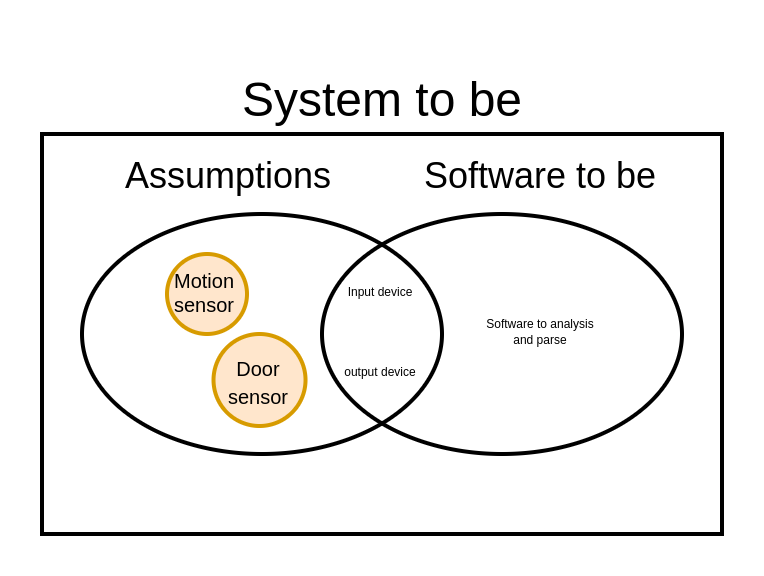
\includegraphics[width=0.5\textwidth]{images/system_to_be.png}
    \caption{مهندسی نیازمندی بیشتر به \lr{Assumption} و قسمت اشتراکی شامل می‌شود.}
    \label{fig: systemToBe}
\end{figure}

\subsubsection{مفهوم \lr{Definition}}

یک معنای دقیق از چیزایی است که می‌نویسم به عبارت دیگر تمام اصطلاحاتی که در سیستم
می‌تواند وجود داشته باشد را بیان می‌کند.

\subsubsection{مفهوم مانیتور کردن}

مانیتور کردن یعنی بررسی داده‌های ورود و انجام تحلیل روی آنها.

\subsubsection{مفهوم کنترل کردن}

کنترل کردن یعنی فرایند بعد از تحلیل، یعنی اعمال کردن نتایج بدست آمده.

\subsubsection{عوامل \lr{Descriptive}}

عوامل توصیفی، قوانین طبیعی و قید و شرط‌های فیزیک که غیر 

\subsubsection{ویژگی دامنه یا \lr{Domain property}}

یک عبارت توصیفی است که یک حقیقت از فیزیک را بیان می‌کند. این عبارت قابل مذاکره
نیست که برای مثال بگوییم بعداً می‌توان آن را تغییر داد. به هیچ وجه نمی‌توان آن
را کم یا زیاد کرد.

برای مثال:

\begin{enumerate}
    \item برای مثال دانشجو نمی‌تواند دو درس مختلف در زمان یکسان اخذ کند. یعنی از
    نظر فیزیک نمی‌توان همزمان در دو کلاس در زمان یکسان حاضر شد. و این پیام را
    نیازمندی نرم‌افزار در حقیقت برنامه نویس مشخص می‌کند.
    \item هنگامی که در‌های قطار بسته باشند، یعنی دیگر باز نیستند.
    \item اگر شتاب قطار مثبت باشد، بدان معانست که سرعت قطار =! صفر می‌باشد.
\end{enumerate}

\subsubsection{دامنه‌ها}

دامنه‌های در دل سازمان‌ها هستند، مانند دامنه پژوهشی، دامنه‌های مالی و ارتباط بین
آدم‌ها در دامنه وجود دارد.

\subsubsection{اسکوپ‌ها}

مجموعه‌هایی از \lr{System requirement} هستند که نرم‌افزار می‌تواند در آنها ورود
داشته باشد. مثلا فعالیت‌های مربوط به ثبت‌نام دانشجو، که اصطلاحاً به آنها
\lr{System scope} می‌گویند. به عبارتی دیگر، مجموعه‌ای از قابلیت‌ها که در
\lr{Domain property} تعریف می‌شود.

\subsubsection*{نکات}

\begin{itemize}
    \item مهندس نیازمندی باید در کنترل و مدیریت اسکوپ‌ها حساسیت داشته باشد که
    نرم‌افزار از دست خارج نشود و باعث پیچیده‌تر شدنش نگردد.
    \item دامنه‌ها درست است که ثابت و غیرقابل مذاکره هستند، اما از یک دامنه به
    دامنه دیگر می‌تواند ویژگی‌ها تغییر کنند در حالی که ساختار این دامنه حفظ شود.
    برای مثال زمانی که دامنه مورد نظر یک کتابخانه فیزیکی است، همزمان دو نفر
    نمی‌توانند یک کتاب مشترک را تقاضا کنند. اما در کتابخانه دیجیتال که به صورت
    اپلیکیشن می‌باشد، درست است که ساختار دامنه همانند موجودیت‌ها و شکل کتابخانه
    فیزیکی است اما نحوه استفاده آن کاملاً تغییر کرده و چندین کاربر می‌توانند
    همزمان یک کتاب را به صورت دیجیتال مطالعه کنند.
    \item در مهندسی نیازمندی تنها یک نمودار استفاده نمی‌شود. برای مثال زمانی که
    یک نمودار \lr{Sequence} برای نمایش ارتباطات دستگاه ها کشیده می‌شود نیازمند
    آن است که نمودار هدف نیز داشته باشد. بعد از آن بایستی تمام ریسک‌های مربوط به
    آن نیز به صورت نمودار اعلام شود. چرا که باعث تولید یک سند مهندسی نیازمندی
    کامل می‌شود که در زمان‌های مختلف می‌توان به آن مراجعه کرد و متوجه تمام
    موضوعات بدون فراموشی تنها یک بخش شد.
    \item بُعد \lr{Why} در نمودار معمولاً نشان‌دهنده اهداف است. مثلا پیاده‌سازی این
    قابلیت هدف‌اش رضایت مشتری است.
    \item همیشه از اهداف شروع می‌کنیم و به نیازمندی‌های سیستمی می‌رسیم و
    نیازمندی سیستمی را در نیازمندی‌های نرم‌افزاری و محیطی بررسی می‌کنیم.
\end{itemize}

\begin{figure}[H]
    \centering
    \begin{forest}
        [Goal
            [
                [System requirement
                    [
                        Software requirement
                    ]
                    [
                        Assumption
                    ] 
                ] 
                [System requirement
                    [
                        Software requirement
                    ]
                    [
                        Assumption
                    ] 
                ] 
            ]
        ]
    \end{forest}
\end{figure}

\subsubsection{تفاوت‌های بین \lr{Descriptive} و \lr{Prescriptive}}

\begin{itemize}
    \item جملات تجویزی را می‌توان برای آنها مذاکره کرد، آنها را کم و زیاد کرد یا
    حتی برای آنها جایگزینی معرفی نمود.
    \item جملات توصیفی اصلاً قابل تغییر نیستند.
\end{itemize}

\subsection{مولفه‌های مربوط به نیازمندی نرم‌افزار در نیازمندی سیستم}

\begin{enumerate}
    \item مانیتورینگ: تمام مقادیر محیطی که نرم‌افزار توسط دستگاه‌های ورودی مانند
    سنسور‌ها، داده‌های آن را دریافت می‌کند.
    \item کنترل: مقادیر محیطی که نرم‌افزار آنهارا می‌تواند از طریق دستگاه‌های
    خروجی (Actuators) آن‌ها را کنترل (اعمال) کند.
    \item مقادیر دستگاه‌های ورودی \footnote{Input}: تمام داده‌هایی که به عنوان
    ورودی در نرم‌افزار استفاده می‌شود.
    \item متغیر‌های خروجی \footnote{Output}: مقادیری که نرم‌افزار آنها را در
    دستگاه‌ّای خروجی اعمال می‌کند.
\end{enumerate}

\subsubsection*{نکته}

بیشتر سازمان‌ها به دو دسته زیر فعالیت‌های خودشان را انجام می‌دهند:

\begin{enumerate}
    \item سازمان‌هایی که هدفگرا هستند و تنها برای رسیدن به محصول آخرین تلاش و
    فعالیت خود را می‌کنند.
    \item سازمان‌هایی که تعداد \lr{Agent} و کاربرانشان زیاد است و ارزش‌های زیادی
    برای آنها قائل می‌شوند به صورت Agentگرا یا عاملگرا هستند.
\end{enumerate}

سطح \lr{System requirement} بالا می‌باشد، چرا که مشتری تنها درخواست می‌کند که
می‌خواهد چنین قابلیت‌هایی وجود داشته باشد، به ماهیت و نیازمندی و حتی پیچیدگی
آنها کاری ندارد.

\subsection{توافق بر لغات}

\begin{enumerate}
    \item \lr{SOFTREQ}: منظور \lr{Software requirement}
    \item \lr{ASM}: منظور مفروضات یا \lr{Assumption}
    \item \lr{DOM}: منظور دامنه یا \lr{Domain}
\end{enumerate}

\begin{equation}
    SOFTREQ + ASM + DOM \rightarrow SYSTEMREQ
\end{equation}

اگر نیازمندی نرم‌افزار، مفروضات و دامنه‌ها همگی مقید و راضی باشند نیازمندی سیستم
نیز بدست می‌آید. با استفاده از پارامتر‌های بالا می‌توان به سیستم نهایی رسید.

\begin{figure}[H]
    \centering
    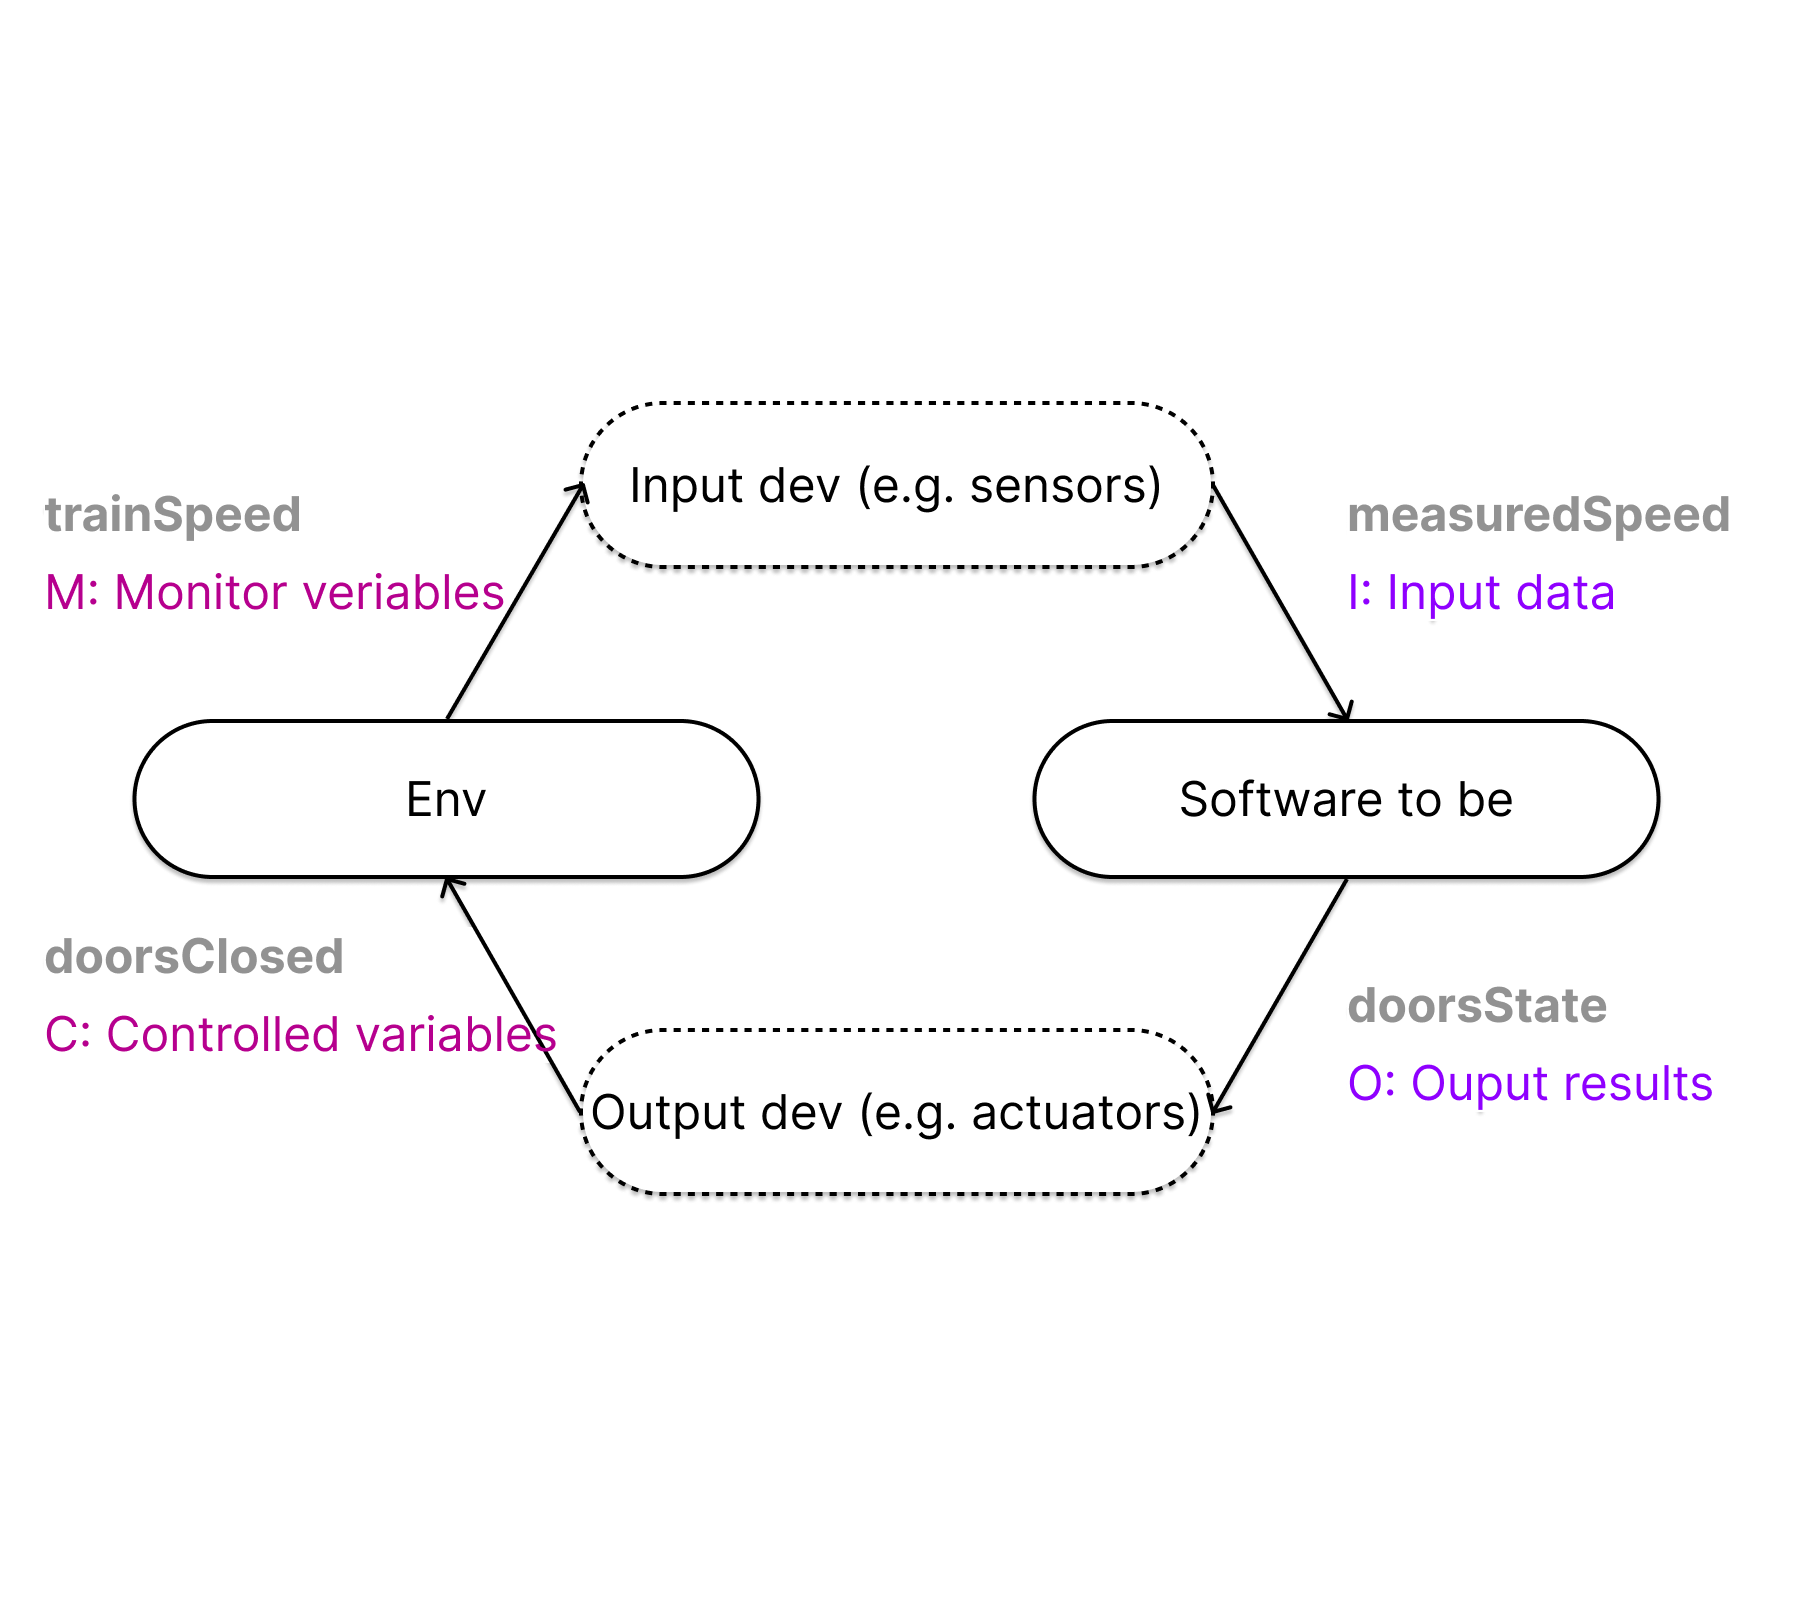
\includegraphics[width=0.7\textwidth]{images/train_sysreq.png}
    \caption{ارتباط نیازمندی سیستم در نرم‌افزار به همراه استدلال‌ها}
    \label{fig: }
\end{figure}


\begin{LTR}
    \begin{itemize}
        \item \lr{SOFTREQ}: Input ` Ouput
        \item \lr{ASM1}: Monitor ` Input
        \item \lr{ASM2}: Ouput ` Control
        \item \lr{SYSREQ}: Monitor ` Control
    \end{itemize}
\end{LTR}

\subsection*{استدلال سناریو}

\begin{equation}
    SOFTREQ: measuredSpeed \neq 0 \rightarrow doorsState = "closed"
\end{equation}

\begin{equation}
    ASM1: measuredSpeed \neq 0 iff trainSpeed \neq 0
\end{equation}

\begin{equation}
    ASM2: doorsState = "closed" iff doorsClosed
\end{equation}

\begin{equation}
    DOM: trainMoving iff trainSpeed \neq 0 
\end{equation}

\begin{equation}
    SYSREQ: trainMoving \rightarrow doorsClosed 
\end{equation}

\subsection{دسته‌بندی نیازمندی‌ها}

\subsubsection{\lr{Functional requirement}}

تعیین می‌کند که چه سرویسی قرار است در \lr{Software to be} ارائه شود. برای مثال:

\begin{itemize}
    \item نرم‌افزار کنترل قطار باید بتواند سرعت تمام بخش‌های سیستم قطار را کنترل
    کند.
    \item سیستم آنلاین فهرست کتب باید براساس موضوع کتاب نام تمام کتابخانه را
    نمایش دهد. 
    \item کاربران در سیستم پارکینگ آنلاین باید بتوانند رزرو لحظه‌ای و رزرو
    روزانه را به انتخاب خودشان استفاده کنند.
    \item دانشجویان زمانی که وارد کلاس آنلاین می‌شوند باید قابلیت به اشتراک
    گذاری صفحه نمایش خود را داشته باشند.
\end{itemize}

همچنین می‌توانند براساس شرایط محیطی باشند که تحت آن چه عملیاتی باید انجام شود:

\begin{itemize}
    \item در‌های قطار تنها در زمانی می‌توانند باز شوند که قطار به طور کامل ایستاده باشد.
\end{itemize}

\subsubsection*{دسته‌بندی توابع}

\begin{enumerate}
    \item \lr{Information}: اطلاع رسانی، اعلانات هر چیزی که قابلیت ارسال و
    دریافت را داشته باشد.
    \item \lr{Satisfaction}: تعیین \lr{State} یک کار است که در جریان معنا دارد.
    \item \lr{Stim-response}: محرک پاسخ، وقتی دکمه در \lr{UI} زده شد آلارم را
    صدا کند.
\end{enumerate}

\subsubsection{\lr{Non-functional requirement}}

تعیین می‌کنند که چگونه یک سرویس می‌تواند ارائه شود. برای این دسته باید مجموعه‌ای
از اقدامات که بار اجرایی دارند را استفاده کرد:

\begin{itemize}
    \item معیار‌ها و نیازمندی‌های کیفی:
    \begin{itemize}
        \item معیار‌های ایمنی
        \item معیار‌‌های امنیتی
        \item سرعت و دقت
        \item عملکرد زمانی و حافظه‌ای
        \item قابلیت استفاده
    \end{itemize}
    \item بقیه موارد
    \begin{itemize}
        \item هنجار‌ها
        \item معماری
        \item نیازمندی‌های توسعه 
    \end{itemize}
\end{itemize}

برای مثال:

\begin{itemize}
    \item دانشجویان هنگام به اشتراک گذاری صفحه خود کیفیت صوت را به خوبی قبل از
    اشتراک گذاری داشته باشند.
    \item قطار هنگام حرکت امکان باز کردن در را نداشته باشد.
    \item دستورات شتاب قطار هر ۳ ثانیه یکبار می‌تواند ارسال شود.
\end{itemize}

\subsection{کیفیت سرویس‌دهی یا \lr{QoS} (محصول)}

پارامتری را نشان می‌دهد که می‌خواهیم آن را از نظر کیفی تامین کنیم. برای مثال
برقراری اهداف امنیتی.

\subsection{\lr{Service Level Agreement}}

یک توافق بین معمار نرم‌افزار و کارفرما برای تعیین سطح سرویس از نظر کیفی می‌باشد.
در قرار‌داد‌های \lr{SLA} مقدار قابل قبولی از \lr{QoS}هایی که دنبالش هستیم را
بیان می‌کنیم.

\subsection{تفاوت بین \lr{Constraint} و \lr{Limitation}}

\lr{Constraint} به معنای قید و شرط است، مقید شدن به چیزی. برای مثال نرم‌افزاری
توسعه داده شود که قابلیت نصب روی دستگاه‌های موبایل را داشته باشد.

\lr{Limitation} به معنای محدودیت است که بار منفی دارد. در این حالت نرم‌افزار
باید با آن کنار بیاید.

\subsection{مفهوم هنجار‌ها یا \lr{Compliance} (محصول)}

منظور از \lr{Compliance} قواعد و هنجار‌هایی است که الزاما ثابت نیستند. نرم‌افزار
باید تابع این هنجار‌ها باشد. قواعدی که در نرم‌افزار قید می‌شود برای مثال فاصله
بین دو ماشین در سال ۲۰۲۰ با تصمیم‌گیری شهرداری برای ماشین‌های خودران ۴ متر توافق
شد. اما بعد از پیشرفت تکنولوزی و علوم مربوطه این فاصله به یک متر کاهش یافت.

\subsection{قید‌های معماری \lr{Architectural constraint} (محصول)}

بعضی از قید‌های معماری مربوط به نصب و راه‌اندازی هستند و برخی دیگر مربوط به
توزیع می‌باشند.

\begin{enumerate}
    \item نصب
    \begin{enumerate}
        \item نرم‌افزار باید روی پلتفرم موبایل یا عینک گوگل قابل نصب باشد
        \item مشخصات لازم برای نصب موفقیت‌آمیز نرم‌افزار و بازی
        \item این نیاز می‌تواند پایین‌تر از سطح سکو نیز باشد، مثلاً نصب تنها در
        یک سیستم عامل مخصوص
        \item قابلیت نصب تنها در سخت‌افزار‌های X86
    \end{enumerate}
    \item قید توزیع: ورودی و خروجی از دو درب مختلف در دانشگاه، به دلیل آنکه
    داده‌های محیطی ورودی و خروجی در دو محل متفاوت است برای رسیدن به توافق در این
    توزیع باید این داده‌ها را در یک جا با هم سینک کنیم تا اطلاعات ورودی و خروجی
    مناسب یکدگیر پدید آید.
\end{enumerate}

\subsection{قید‌های توسعه \lr{Development constraint} (مدیر پروژه)}

یکی از مهم‌ترین عوامل نگرانی مدیر پروژه است، کاری به ماهیت محصول ندارد بلکه برای
او مهم‌ترین عوامل انتخاب مناسب متدولوژی و تصمیم درست می‌باشد. تعیین هزینه زمانی
و مالی نیز از دیگر نگرانی‌های مدیر پروژه می‌باشد تا در نهایت طراح معماری بتواند
با دید کامل و بدون تحت فشار قرار گرفتن، معماری مناسب را طراحی کند.

\subsection{فرایند و مراحل مهندسی نیازمندی‌}

برای ساخت سبد دامنه خود نیازمند انجام فرایند مهندسی نیازمندی هستیم. این فرایند
چهار قدم اصلی را بیان می‌کند. مهم‌ترین ویژگی این فرایند مراحل آن هستند که
می‌توانند به صورت تکرار پذیر انجام شوند. حرکت در بین این فرایند به صورت ساعتگرد
می‌باشد.

\begin{figure}[H]
    \centering
    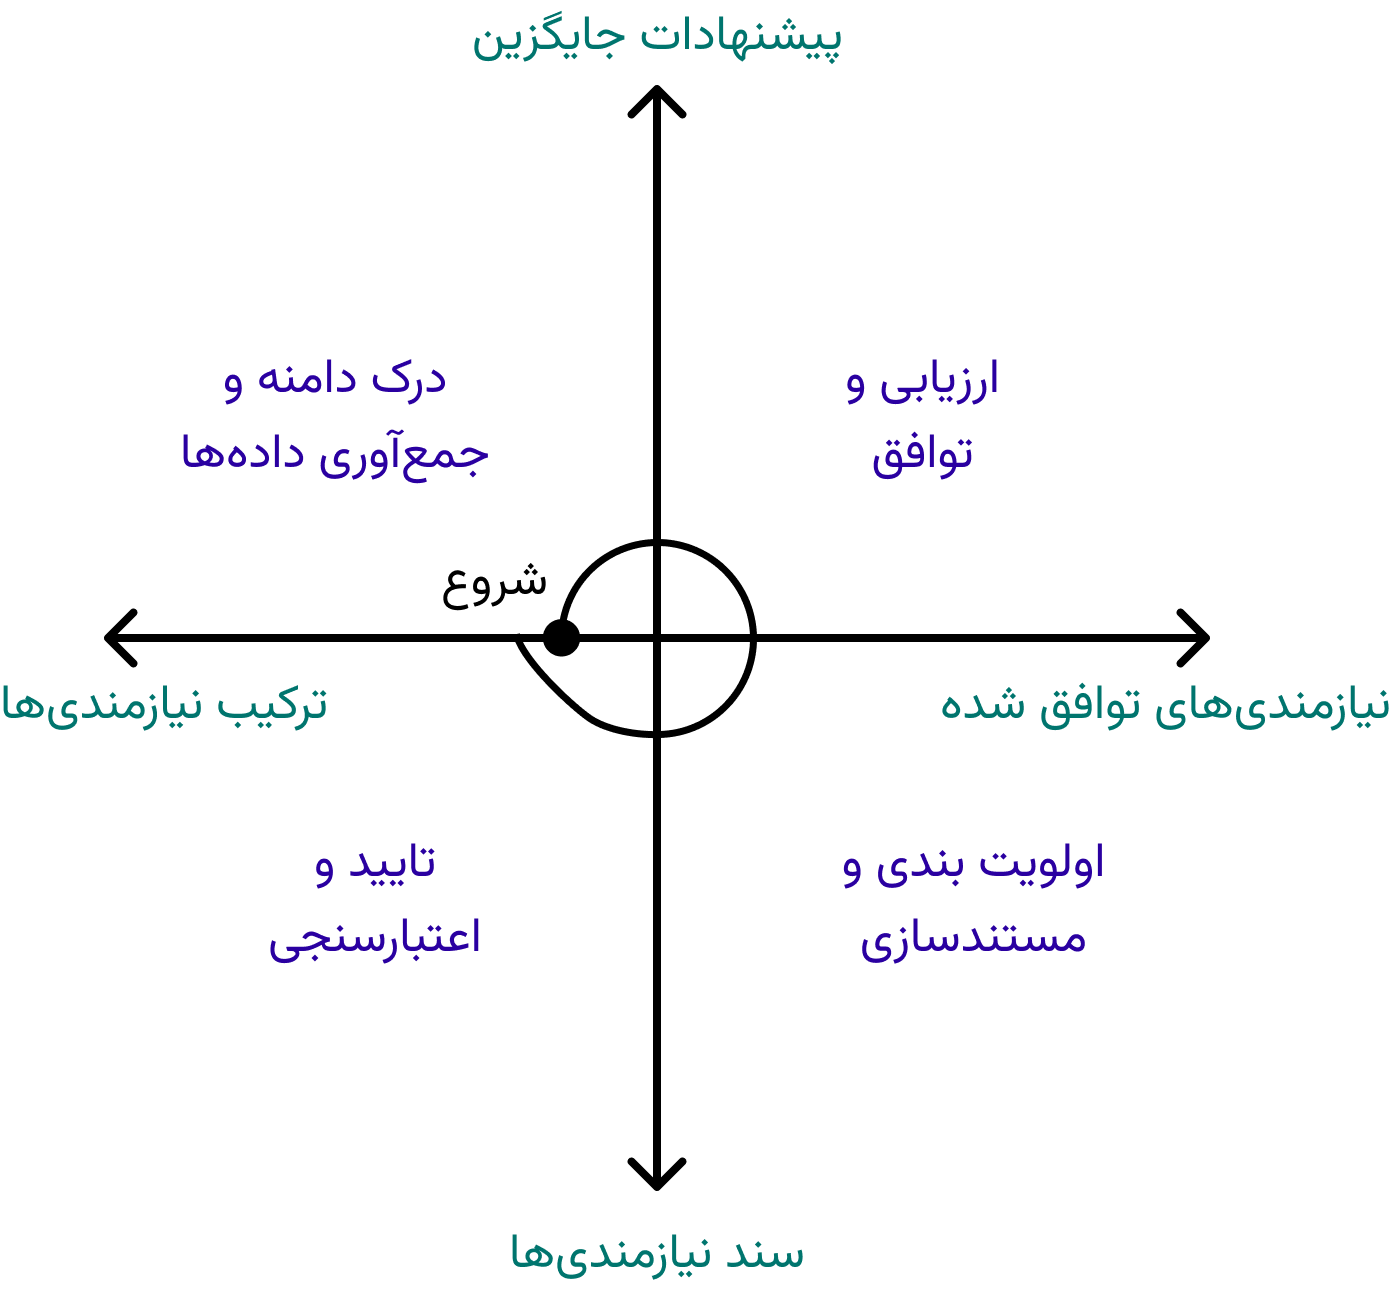
\includegraphics[width=0.5\textwidth]{images/re_process.png}
    \caption{مراحل مهندسی نیازمندی‌ها}
    \label{fig: reProcess}
\end{figure}

\subsubsection{پیشنهادات جایگزین، درک دامنه و جمع‌آوری داده‌ها}

این بخش با دامنه‌ها و استخراج نیازمندی‌ها ارتباط دارد. یعنی مهم‌ترین وظیفه در
این ناحیه جمع‌آوری داده‌ها می‌باشد. سعی می‌کنیم تمام سناریو‌ها را بررسی کنیم و
به لیستی از داده‌های در رابطه با دامنه خواسته‌های مشتری برسیم. به یاد داشته
باشیم که داده‌های جمع‌آوری شده صرفا همه آنها مفید نمی‌باشد پس نتیجه می‌گیریم که
این لیست قابل تغییر و حذف می‌باشد که به داده‌های اصلی برسیم. برای مثال وقتی در
حال جمع‌آوری داده برای توسعه سیستم مالی هستیم با داده‌های بخش بایگانی هم رو به
رو خواهیم شد که هیچ ارتباط مستقیمی با سناریو‌های مالی ندارد پس می‌توانیم از
جمع‌آوری داده در بخش بایگانی صرف نظر کنیم.

\subsubsection{نیازمند‌های توافق شده، ارزیابی و توافق}

همانطور که از نامش پیداست در این ناحیه به تجزیه و تحلیل و ارزیابی داده‌ها
می‌پردازیم. به گونه‌ای که سعی می‌کنیم داده‌هایی که نامربوط به \lr{Scope} می‌باشد
را شناسایی کنیم و آنها را حذف کنیم. هر خواسته‌ای در \lr{Scope} مشتری می‌تواند
ریسک‌هایی باشد که به عنوان قابلیت در نرم‌افزار می‌خواهد پیاده شود.

\begin{itemize}
    \item قضیه برنامه \lr{LMS} را در نظر داشته باشید. کلاس آنلاین به حضور
    دانشجویان نیاز دارد و قابلیت‌هایی در خصوص عضویت آنها در این سامانه وجود دارد
    اما ریسکی که در این میان به وجود می‌آید آن است که ممکن است اینترنت قطع شود و
    دسترسی دانشجویان به این سامانه با مشکل مواجه شود.
\end{itemize}

سوالی که در این میان مطرح می‌شود آن است که آیا تمام نیازمندی‌هایی که به سیستم
وارد می‌شود الزاماً هم‌راستا می‌باشد؟

پاسخ به این سوال خیر می‌باشد چرا که ممکن است نیاز دو \lr{Assumption} با یکدیگر
تداخل داشته باشد.

\begin{itemize}
    \item قضیه کارنامه را به یاد داشته باشید. درخواست مشتری اول (استاد) آن است
    که فقط او بتواند در هنگام ثبت نمره کارنامه را دسترسی داشته باشد. در راستای
    آن مشتری دوم (دانشجو) هم دقیقاً همین نیاز را دارد. این دو نیاز هم‌راستا
    نمی‌باشد چرا که اگر یکی را تنها برای یک نوع مشتری برآورده کنیم ممکن است با
    مشتری دیگر تداخل یا \lr{Conflict} ایجاد شود.
\end{itemize}

\subsubsection{سند نیازمندی‌ها، اولویت‌بندی و مستندات}

وقتی به این مرحله رسیده‌ایم یعنی با دو مرحله قبلی در نیازمند‌های مشتری به اجماع
رسیده‌ایم. یک سبدی از \lr{Scope}ها که خیلی آشفته بود به یک سبدی تبدیل می‌شود که
همه افراد روی آن توافق دارند. این توافق‌ها در سند نیازمندی نوشته می‌شوند. این
سند یک قالب استاندارد دارد و در این قالب مشخص می‌شود که با چه ابزاری باید کار
کنیم، چگونه بنویسیم و نماد بصریمان به چه شکلی باشد. بعد از این توافق‌ها این سند
به طراح معماری نرم‌افزار تحویل داده می‌شود. این سند با نمودار‌های بصری‌اش زبان
مشترک بین طراح و مهندس نیازمندی است تا مطالب صریح و سریع به طراح معماری منتقل
شود.

\subsubsection{نیازمندی‌های ترکیبی،‌ تایید و اعتبارسنجی}

سبدی که تا الان آماده شده است می‌تواند دستخوش تغییرات باشد تا به حدی که به ۸۰
درصد نیازمندی‌های ثابت و ۲۰ درصد نیازمندی‌هایی که باید تغییر کنند یا بروز شوند.
این تغییر ۲۰ درصدی می‌تواند بخش‌های صحیح را هم تحت تاثیر خودش قرار دهد (اشاره به
قضیه \lr{Side effect}). پس در هر بار ایجاد تغییر در نیازمندی‌ها بایستی در ابتدا
اعتبارسنجی شوند و تایید ایجاد تغییرات را دریافت کند.

\subsubsection*{نکته}

مراحل نیازمندی‌ها می‌تواند چندین دور حلقوی داشته باشد تا همه موارد دخیل در آن به
نسخه پایدار خود برسند.

\subsection{نیازمندی‌ها در چرخه توسعه نرم‌افزار}

سوال: آیا هر سیستمی نیازمند مهندسی نیازمندی می‌باشد؟

خیر، سند نیازمندی برای سازمان‌ها با سیستم بزرگ (سیستم‌های \lr{Legacy}) کاملاً
مورد احتیاج می‌باشد. به طور کل سازمان‌هایی که جریان کاری (\lr{Workflow}) اصلی را
اداره می‌کنند نیازمند سند نیازمندی هستند. پروژه‌های استارتاپی که به مردم خدمت
می‌کنند در اصل جنس خدمت با دیگر سازمان‌ها یکی است اما نحوه انجام آن متفاوت
می‌باشد. این سیستم‌ها هم سند نیازمندی برایشان اهمیت دارد.

به خاطر داشته باشید که سند نیازمندی قابلیت استفاده مجدد را به پروژه‌های مشابه
می‌دهد. به طور کلی گفتنی است که سند نیازمندی یک منبعی برای پروژه‌های مشابه
می‌باشد نه یک الگو.

به طور کلی، در سند نیازمندی، خواسته‌های مشتری تحلیل و جمع‌آوری می‌شود و بعد
قرارداد در پروژه پیاده‌سازی می‌شوند.

\subsection{\lr{Request for Proposal} یا \lr{RFP}}

سازمان‌ها بر اساس \lr{RFP} کار می‌کنند. مهندس نیازمندی و متخصصین با هم روی این
سند بر اساس خواسته‌های مشتری توافق می‌کنند که کار خودشان را شروع کنند. معمولاً
واحد‌های \lr{IT} مسئول این اسناد هستند.

\subsection{تعریف: به اجماع رسیدن مطالب از سند نیازمندی}

سند نیازمندی یا \lr{Requirement Document} محصول اصلی فرایند مهندسی نیازمندی است.
در آن سیستمی که می‌خوایم در آینده داشته باشیم (\lr{System-to-be}) به شکل اهداف
\footnote{\lr{Objectives}}، قید و بند‌ها \footnote{\lr{Constraints}}، مفاهیم
ارجاع داده شده، تسک‌ها و تکالیف مشخص شده، نیازمندی‌ها، فرضیات
\footnote{\lr{Assumption}} و ویژگی دامنه‌های مربوطه تعریف شده است.

\subsection{تاثیراتی که سند نیازمندی به فرآورده‌های نرم‌افزاری دارد}

\subsubsection{\lr{Prototype}}

بعد از جمع‌آوری داده‌ها به عنوان ورودی به سیستم آینده \lr{(System to be)}، یک
نمونه آزمایشی یا \lr{Prototype} که اصطلاحاً به آن \lr{Mock-up} هم گفته می‌شود،
را طراحی و آماده می‌کنیم تا بتوانیم نیاز‌هایی که از مشتری در نسخه اول سند
نیازمندی دریافت کرده‌ایم را به طور کاملاً اولیه پیاده‌سازی کنیم تا بازخورد مشتری
را در رابطه با آن دریافت کنیم. دلیل دو طرفه بودن این بخش با سند نیازمندی آن است
که بررسی کنیم آیا نیاز‌هایی که به ما منتقل شده است صریح و مناسب با درخواست‌های
مشتری بوده است؟ ممکن است نیاز شود برخی از موارد حذف یا حتی موارد جدید را اضافه
کنیم تا سبد \lr{Scope} ما تکمیل شود. نکته مهم آن است که \lr{Prototype} می‌تواند
در سطح \lr{Functional} باشد و هم در سطح \lr{Non-functional}. البته باید در نظر
داشت که همیشه \lr{Prototype} لزومی ندارد که به صورت کامل آماده شود، بلکه ممکن
است در خصوص برخی از نیازمندی‌ها که مبهم است یک \lr{Prototype} درست کنیم.

\subsubsection{\lr{Project estimations (Size, Cost, Shedules)}}

یکی از نیازمندی‌های غیرعملیاتی مربوط به توسعه است که روی سبد \lr{Scope}ها تاثیر
گذار می‌باشد. در این قسمت رابطه سند نیازمندی با آن دو طرفه می‌باشد تا مشخص کنیم
برای نیازمندی‌های خود چقدر زمان، چه مقدار هزینه و چه تعداد نیروی انسانی به طور
مثال تعیین کنیم. در این قسمت سند نیازمندی ممکن است چند بار دستخوش تغییرات قرار
گیرد و اصطلاحاً نسخه‌بندی شود. ممکن است در نسخه اولیه نیاز ما با زمان مطابقت
داشته باشد اما به علت بزرگ شدن پروژه و بروز شدن خواسته‌های مشتری، دیگر این زمان
با نیازمندی‌های جدید سازگاری ندارد و بایستی بروز شود.

\subsubsection{\lr{Acceptance test}}

این مورد رابطه یک طرفه با سند نیازمندی‌ها دارد، چرا که نیازمندی‌ها در این مرحله
به درستی تنظیم شده‌اند و بعد از آن توسط معمار نرم‌افزار پیاده‌سازی صورت گرفته
است. پس نیازمند مجموعه‌ای از سناریو‌ها هستیم تا بررسی کنیم که نیازمندی‌ها با
خواسته‌های مشتری مطابقت داشته است یا خیر. سناریو‌های تست از سند نیازمند‌ها طراحی
و آماده می‌شود.

\subsubsection{\lr{Architectural design}}

طراحی معماری نرم‌افزار به طور مشخص با نیازمندی‌های نرم‌افزار در ارتباط است که
ممکن است تاثیر به سزایی بر روی نیازمندی‌های \lr{Non-functional} داشته باشد. بر
این اساس، سند نیازمندی‌ها ورودی اساسی برای طراحی معماری نرم‌افزار از دیدگاه‌های
زیر می‌باشد:

\begin{itemize}
    \item شناسایی معماری کامپوننت‌ها و اتصالات
    \item مشخصات آنها که در سند نیازمندی مطرح می‌شود.
    \item مجموعه‌ای از سبک‌های معماری نرم‌افزار
    \item ارزیابی گزینه‌های معماری نرم‌افزار در برابر نیازمندی‌های \lr{Non-functional}
\end{itemize}

\subsubsection{\lr{Software quality assurance}}

رابطه یک طرفه با سند نیازمندی‌ها دارد به گونه‌ای که سند نیازمندی‌ها مراجع نهایی
را برای فعالیت‌های اطمینان کیفیت ارائه می‌دهد.

\begin{itemize}
    \item نیازمندی‌ها اساسی را برای تست داده‌ها و پذیرش آنها ارائه می‌دهد.
    \item این اساس‌ها به عنوان یک سری چک لیست برای بررسی نرم‌افزار استفاده
    می‌شوند.
\end{itemize}

% \subsubsection{\lr{Implementation and integration}}

% \subsubsection{\lr{Documentation}}

% \subsubsection{\lr{Maintenance}}

% ریپورت صفحه ۵۳ نمودار رو نگاه اینجا بنویس.

% expectation منظور همان Assumptionهاست.
